\documentclass[11pt,a4paper]{article}
\usepackage[utf8]{inputenc}
\usepackage[vietnamese]{babel}
\usepackage{amsmath,amssymb}
\usepackage[version=4]{mhchem}
\usepackage{geometry}
\geometry{top=0.65cm,bottom=0.65cm,left=1.25cm,right=1.25cm,headheight=20pt,headsep=3pt,footskip=9pt}
\usepackage{graphicx}
\usepackage{xcolor}
\usepackage{tabularx}
\usepackage{array}
\usepackage{tikz}
\usepackage{multicol}
\usepackage{fancyhdr}
\usepackage{enumitem}

\definecolor{hfRed}{HTML}{D32F2F}
\definecolor{hfGreen}{HTML}{8BC390}
\definecolor{mainGreen}{HTML}{2E7D32}

\usepackage{ex_test}

\pagestyle{fancy}
\fancyhf{}
\renewcommand{\headrulewidth}{0.75pt}
\renewcommand{\headrule}{\hbox to\headwidth{\color{hfGreen}\leaders\hrule height \headrulewidth\hfill}}
\renewcommand{\footrulewidth}{0.75pt}
\renewcommand{\footrule}{\hbox to\headwidth{\color{hfGreen}\leaders\hrule height \footrulewidth\hfill}}

\fancyhead[L]{\small\itshape\color{hfRed}Tài liệu lưu hành nội bộ}
\fancyhead[R]{\small\color{hfRed}Thầy \textbf{TRẦN VĂN THẠNH} - 0777.470.803}

\fancyfoot[L]{\footnotesize\itshape\color{hfRed}CS1: 6/15 Nguyễn Hoàng, P. Kim Long, TP Huế \quad|\quad CS2: 24 Đặng Thái Thân, TP Huế}
\fancyfoot[R]{\small\textbf{\color{hfRed}Trang \thepage}}

\setlength{\parindent}{0pt}
\setlength{\parskip}{0.0pt}

\def\loigiai#1{}

\begin{document}
\Opensolutionfile{ans}[ans-de18-hs]

\noindent
\begin{minipage}[t]{0.48\textwidth}
	\textbf{SỞ GIÁO DỤC VÀ ĐÀO TẠO THỪA THIÊN HUẾ}\\
	\textbf{TRƯỜNG THPT HAI BÀ TRƯNG}\\
	\textbf{ĐỀ CHÍNH THỨC}\\
	\textit{(Đề thi có 04 trang)}
\end{minipage}\hfill
\begin{minipage}[t]{0.48\textwidth}
	\raggedleft
	\textbf{\color{mainGreen}ĐỀ KIỂM TRA ĐỊNH KỲ CHƯƠNG 6 (ĐẠI CƯƠNG KIM LOẠI)}\\
	\textbf{MÔN: HOÁ HỌC -- LỚP 12}\\
	\textit{Thời gian làm bài: 50 phút (không kể thời gian phát đề)}\\
	\textbf{Mã đề thi: 118}
\end{minipage}


\vspace{1pt}
\noindent\textit{Họ, tên thí sinh: \dots\dots\dots\dots\dots\dots\dots\dots\dots\dots\dots\dots\dots\dots\dots\dots\dots\dots\dots\dots\dots\dots Lớp: \dots\dots\dots\dots SBD: \dots\dots\dots\dots}\\
\noindent\textit{(Cho biết nguyên tử khối: H = 1; C = 12; N = 14; O = 16; Na = 23; Mg = 24; Al = 27; S = 32; Cl = 35,5; K = 39; Ca = 40; Fe = 56; Cu = 64; Zn = 65; Br = 80; Ag = 108; Ba = 137; Au = 197; Pb = 207; hằng số Faraday F = 96485 C/mol).}

\vspace{1pt}
\noindent
\textbf{PHẦN I (4,5 điểm -- 18 câu): Câu trắc nghiệm nhiều phương án lựa chọn.}\\
\textit{Thí sinh trả lời từ câu 1 đến câu 18. Mỗi câu hỏi thí sinh chỉ chọn một phương án.}

\begin{ex}
Ở điều kiện thường, kim loại nào sau đây ở trạng thái lỏng?
\choice
{Au.}
{Cu.}
{Na.}
{Hg.}
\loigiai{}
\end{ex}

\begin{ex}
Kim loại có độ cứng lớn nhất là
\choice
{Cr.}
{Al.}
{Mg.}
{Na.}
\loigiai{}
\end{ex}

\begin{ex}
Kim loại có nhiệt độ nóng chảy cao nhất là
\choice
{Na.}
{Pb.}
{Hg.}
{W.}
\loigiai{}
\end{ex}

\begin{ex}
Kim loại có khối lượng riêng nhỏ nhất là
\choice
{Na.}
{Li.}
{Fe.}
{Al.}
\loigiai{}
\end{ex}

\begin{ex}
Trong mạng tinh thể kim loại chứa các cation kim loại được sắp xếp theo một trật tự nhất định cùng với các electron chuyển động
\choice
{theo một quỹ đạo xác định.}
{xung quanh một vị trí xác định.}
{tự do trong toàn bộ mạng tinh thể.}
{trong một khu vực không gian nhất định.}
\loigiai{}
\end{ex}

\begin{ex}
Hình dưới đây mô tả tính chất vật lí nào của kim loại? (hình tròn to mô tả ion kim loại, hình tròn nhỏ mô tả electron tự do)
\par\vspace{1pt}\centerline{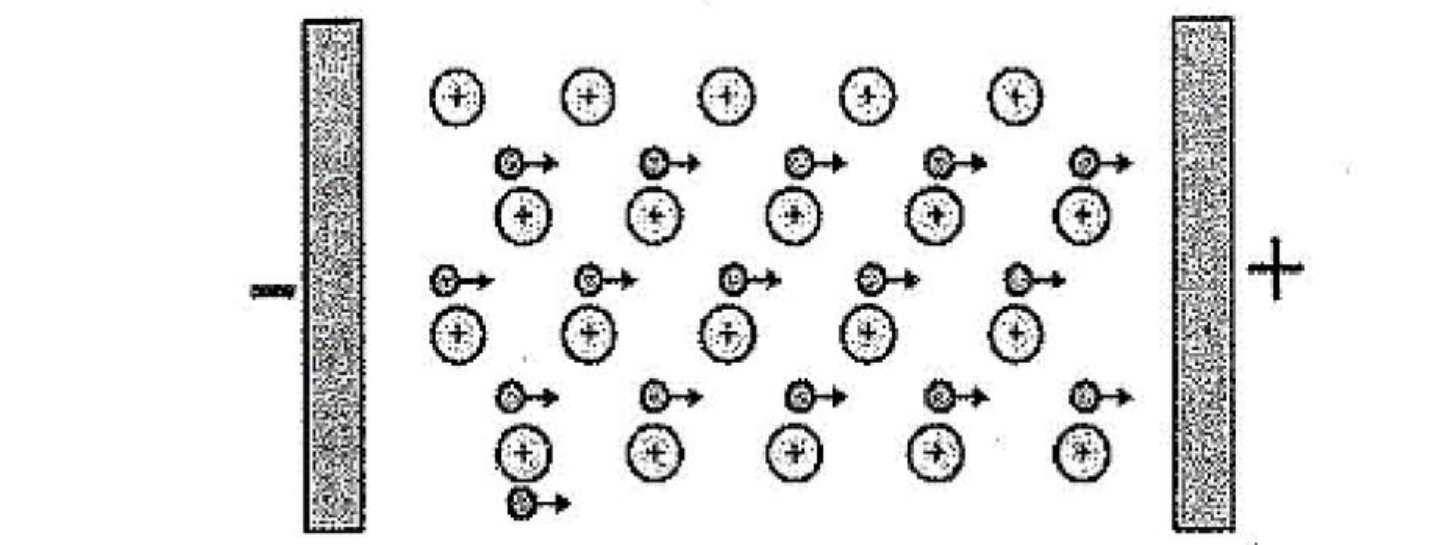
\includegraphics[height=1.4cm]{images_crop_de18/p1_cau6_tinh_dan_dien.png}}\vspace{1pt}
\choice
{Tính dẻo.}
{Tính dẫn điện.}
{Tính dẫn nhiệt.}
{Tính cứng.}
\loigiai{}
\end{ex}

\begin{ex}
Cầu chì là một phần tử hay thiết bị bảo vệ mạch điện bằng cách làm đứt mạch điện. Cầu chì được sử dụng nhằm phòng tránh các hiện tượng quá tải trên đường dây. Dây cầu chì thường được làm bằng kim loại chì (Pb), thiếc trắng (Sn) hoặc cadmium (Cd).
\par\vspace{1pt}\centerline{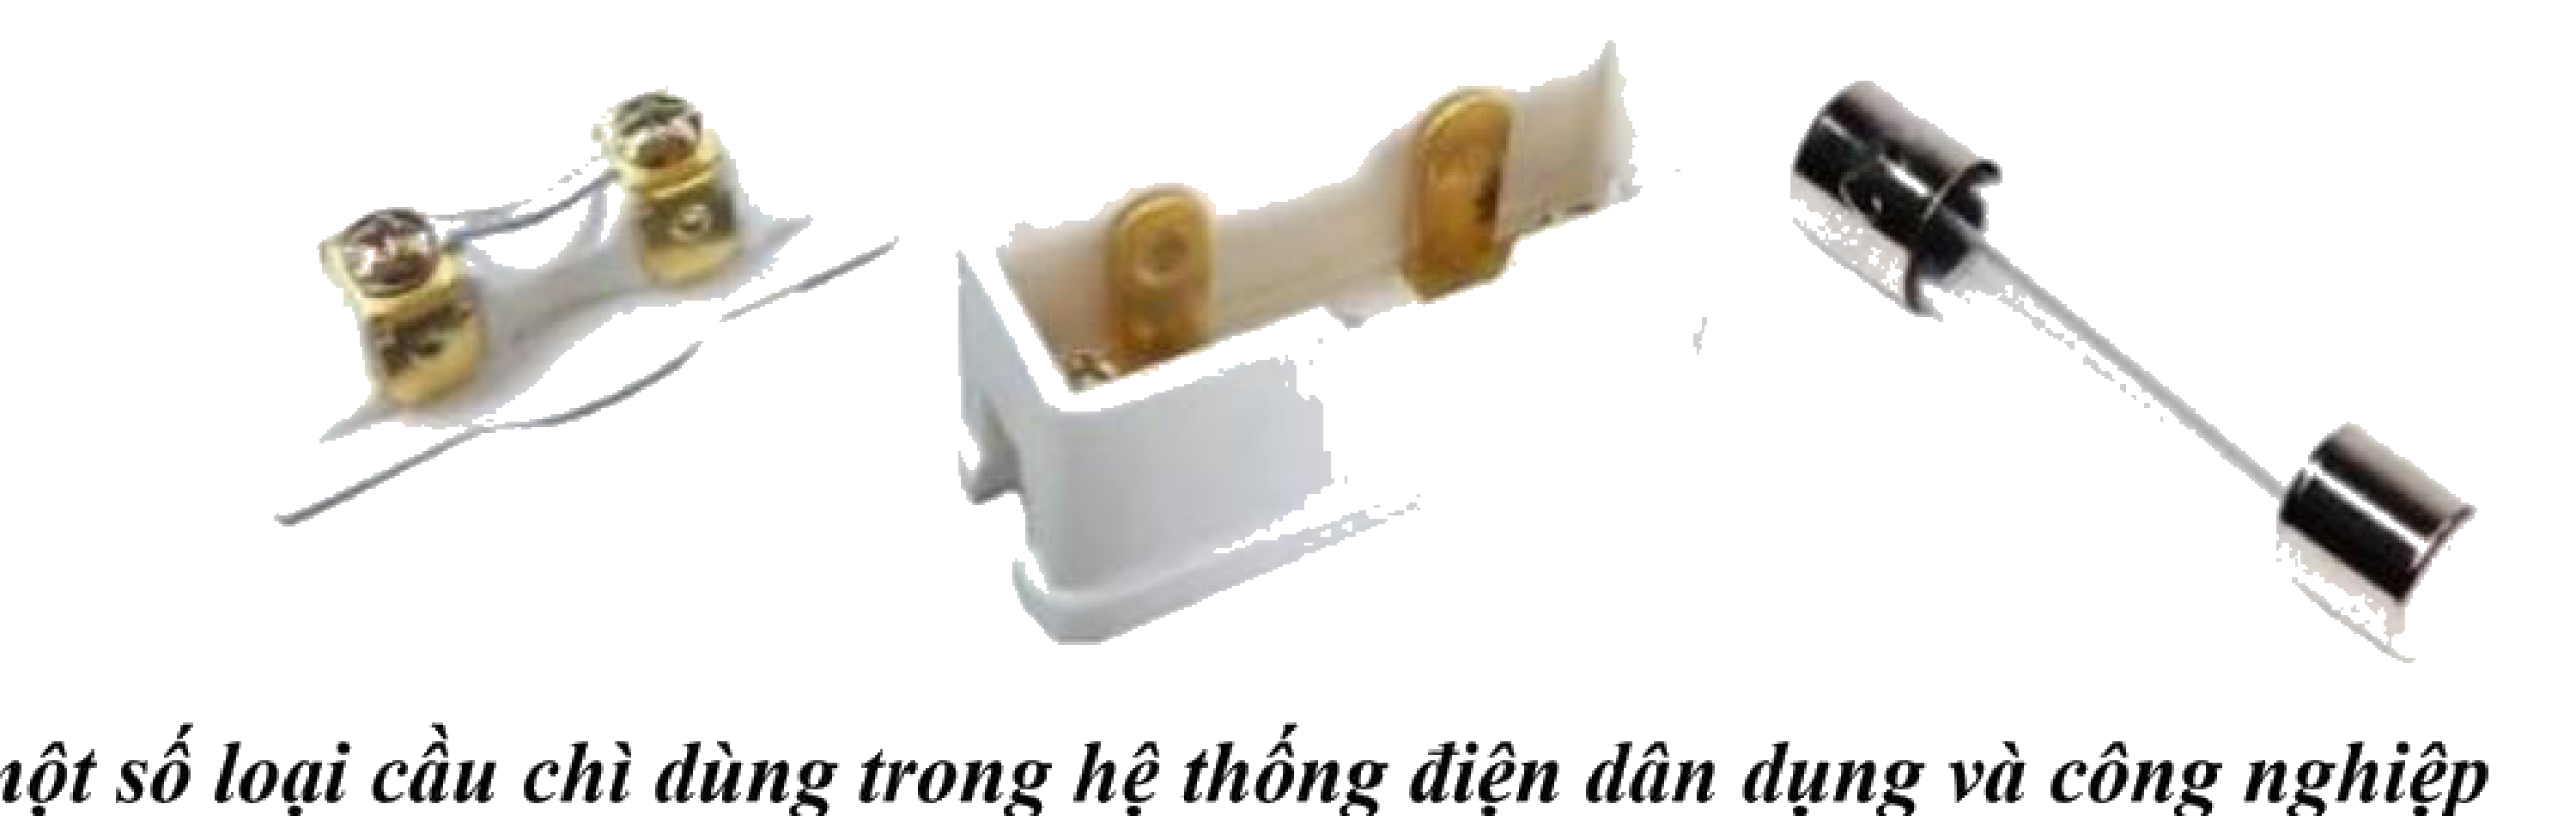
\includegraphics[height=1.4cm]{images_crop_de18/p1_cau7_cau_chi.png}}\vspace{1pt}
Ứng dụng này dựa trên tính chất nào của các kim loại trên?
\choice
{Có tính dẻo cao.}
{Có nhiệt độ nóng chảy tương đối thấp.}
{Có độ dẫn điện cao.}
{Có độ cứng tương đối thấp.}
\loigiai{}
\end{ex}

\begin{ex}
Trong nước nguyên chất khi phản ứng xảy ra sẽ có quá trình sau:\\
$\ce{2H2O + 2e -> H2 + 2OH-} \quad E^\circ_{\ce{2H2O/H2 + 2OH-}} = -0{,}42\text{ V}$.\\
Cho $E^\circ_{\ce{Na+/Na}} = -2{,}71\text{ V}$; $E^\circ_{\ce{Cu^2+/Cu}} = +0{,}34\text{ V}$; $E^\circ_{\ce{Mg^2+/Mg}} = -2{,}36\text{ V}$; $E^\circ_{\ce{Al^3+/Al}} = -1{,}68\text{ V}$.\\
Hãy cho biết kim loại nào sau đây \textbf{không} phản ứng được với nước ở điều kiện chuẩn.
\choice
{Cu.}
{Na.}
{Mg.}
{Al.}
\loigiai{}
\end{ex}

\begin{ex}
Cho các kim loại: Na, Ca, Cu, Ag, K. Số kim loại có khả năng khử được nước ở điều kiện thường giải phóng \ce{H2} là
\choice
{2.}
{1.}
{4.}
{3.}
\loigiai{}
\end{ex}

\newpage

\begin{ex}
Lấy một đinh sắt đã được làm sạch bề mặt rồi ngâm vào dung dịch \ce{CuSO4} một thời gian. Hiện tượng nào sau đây \textbf{không} xuất hiện trong thí nghiệm trên?
\choice
{Có chất rắn màu đỏ bám lên đinh sắt.}
{Màu xanh của dung dịch nhạt dần.}
{Có bọt khí thoát ra mạnh trên bề mặt đinh sắt.}
{Đinh sắt bị ăn mòn một phần.}
\loigiai{}
\end{ex}

\begin{ex}
Nguyên tắc chung để điều chế kim loại từ hợp chất của chúng là
\choice
{khử cation kim loại thành kim loại.}
{oxi hoá ion kim loại thành kim loại.}
{oxi hoá kim loại thành ion kim loại.}
{khử kim loại thành ion kim loại.}
\loigiai{}
\end{ex}

\begin{ex}
Gang và thép là hai hợp kim quan trọng nhất của sắt. Chúng có rất nhiều ứng dụng trong đời sống và sản xuất. Để sản xuất gang, người ta khử oxide của sắt (\ce{Fe2O3} hoặc \ce{Fe3O4}) trong quặng sắt bằng khí CO (được tạo ra do đốt cháy than cốc). Sắt được tạo ra trong quá trình sản xuất gang bằng phương pháp nào?
\choice
{Kết tinh.}
{Nhiệt luyện.}
{Thuỷ luyện.}
{Chiết.}
\loigiai{}
\end{ex}

\begin{ex}
Kim loại kẽm (zinc, Zn) được sản xuất trong công nghiệp từ quặng sphalerite (có thành phần chính là ZnS) theo sơ đồ: $\ce{ZnS} \xrightarrow{+\ce{O2},\, t^\circ} \ce{ZnO} \xrightarrow{+\ce{C},\, t^\circ} \ce{Zn}$. Phương pháp điều chế kim loại nào đã được sử dụng trong quá trình sản xuất zinc theo sơ đồ trên?
\choice
{Thuỷ luyện.}
{Nhiệt luyện.}
{Điện phân.}
{Kết tinh.}
\loigiai{}
\end{ex}

\begin{ex}
Vàng (Au) tồn tại trong tự nhiên ở dạng đơn chất. Tuy nhiên, hàm lượng Au trong quặng thường rất thấp nên rất khó tách Au bằng cơ học. Trong công nghiệp, người ta tách vàng từ quặng theo sơ đồ sau:\\
Quặng chứa vàng $(\ce{Au}) \xrightarrow{+\ce{O2} + \ce{KCN} + \ce{H2O}} \ce{K[Au(CN)2]} \text{ (aq)} \xrightarrow{+\ce{Zn dư}} \ce{Au} \text{ (s)}$\\
Phương pháp điều chế kim loại nào đã được sử dụng trong sơ đồ trên?
\choice
{Thuỷ luyện.}
{Nhiệt luyện.}
{Điện phân.}
{Chiết.}
\loigiai{}
\end{ex}

\begin{ex}
\begin{minipage}[t]{0.72\textwidth}
Thực hiện thí nghiệm sau:\\
\textbf{Bước 1:} Cho dung dịch \ce{NaCl} 5\% vào ống chữ U như hình bên.\\
\textbf{Bước 2:} Nhúng thanh Cu và thanh Zn đã làm sạch vào 2 đầu ống.\\
\textbf{Bước 3:} Nối hai thanh kim loại bằng dây dẫn.\\
Sau bước 2, kim loại nào bị ăn mòn?
\end{minipage}\hfill
\begin{minipage}[t]{0.26\textwidth}
\centering
\vspace{-4pt}
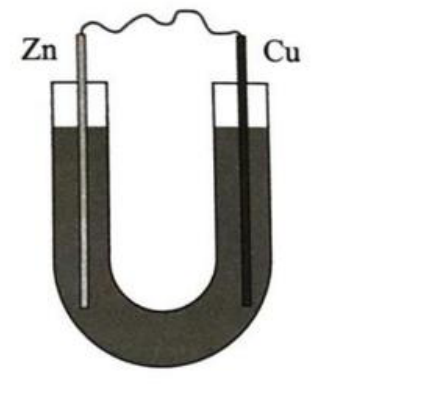
\includegraphics[height=1.55cm]{images_crop_de18/p1_cau15_u_tube.png}
\end{minipage}
\choice
{Đồng.}
{Cả hai đều bị ăn mòn.}
{Kẽm.}
{Không kim loại nào bị ăn mòn.}
\loigiai{}
\end{ex}

\begin{ex}
Để khảo sát quá trình ăn mòn kim loại, tiến hành ba thí nghiệm như hình dưới đây. Mỗi ống nghiệm chứa một chiếc đinh sắt trong các môi trường khác nhau. Phát biểu nào dưới đây là đúng?
\par\vspace{1pt}\centerline{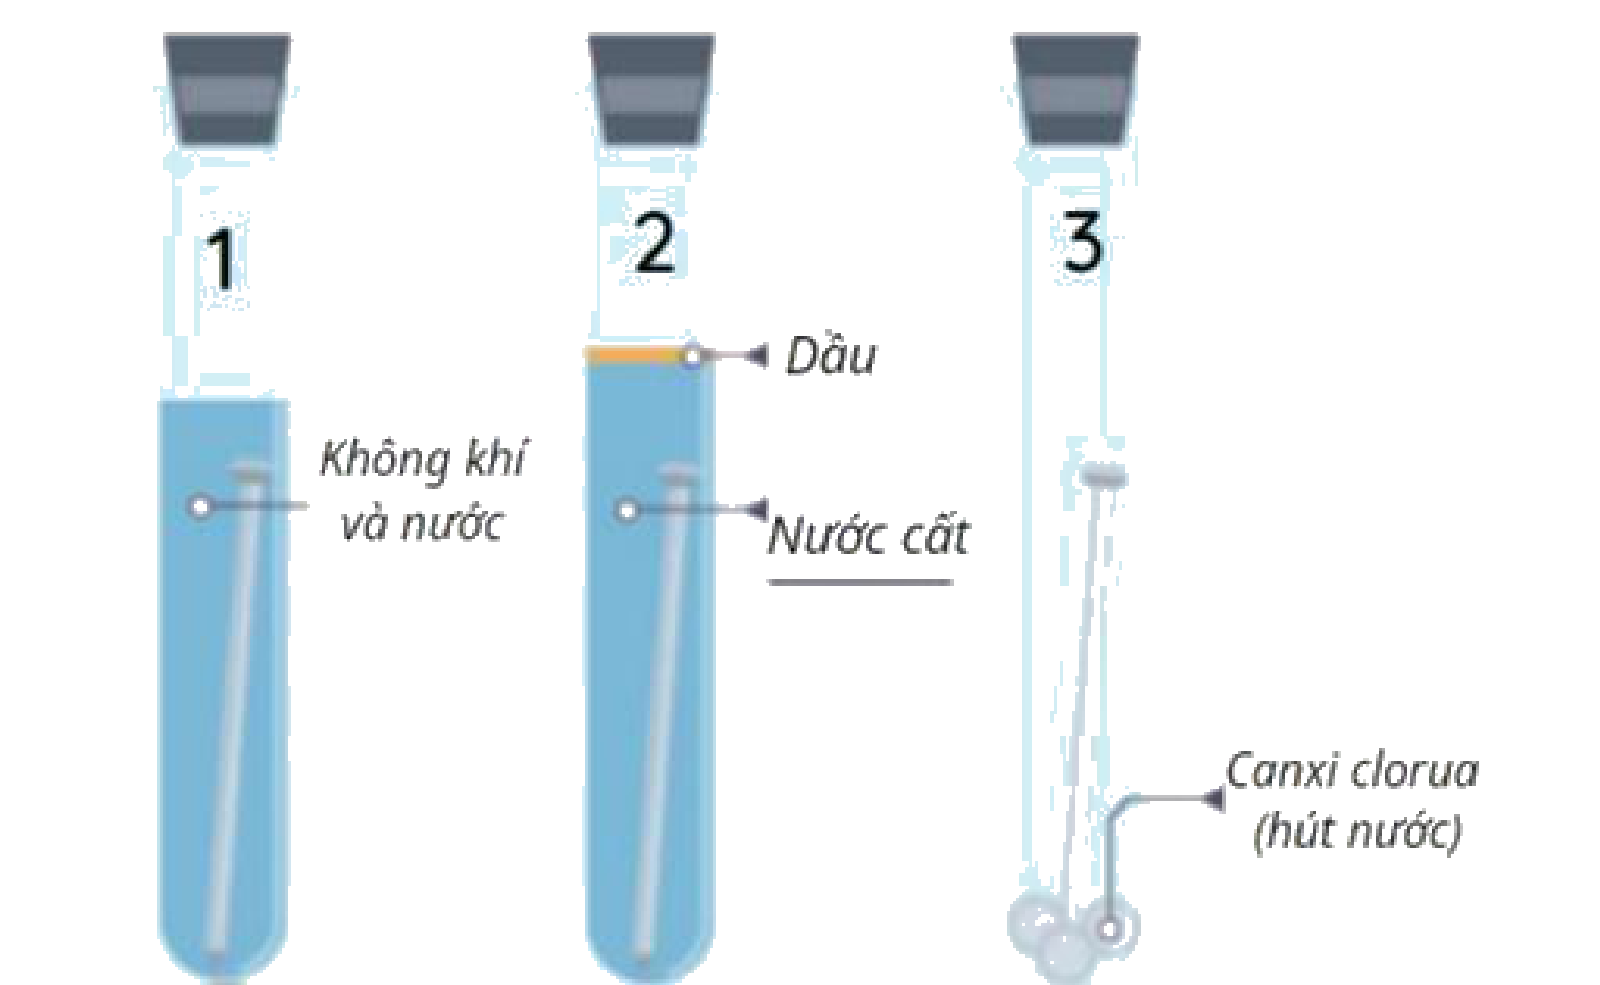
\includegraphics[height=1.5cm]{images_crop_de18/p1_cau16_an_mon_ong_nghiem.png}}\vspace{1pt}
\choice
{Sau một thời gian, đinh sắt trong cả ba ống nghiệm đều bị gỉ.}
{Sau một thời gian, đinh sắt trong cả ba ống nghiệm đều không có sự thay đổi.}
{Sau một thời gian, đinh sắt trong ống nghiệm số 1 và 3 bị gỉ.}
{Sau một thời gian, chỉ có đinh sắt trong ống nghiệm số 1 bị gỉ.}
\loigiai{}
\end{ex}

\begin{ex}
Trong số các thí nghiệm sau đây, thí nghiệm nào có tốc độ ăn mòn đinh sắt chậm nhất?
\par\vspace{1pt}\centerline{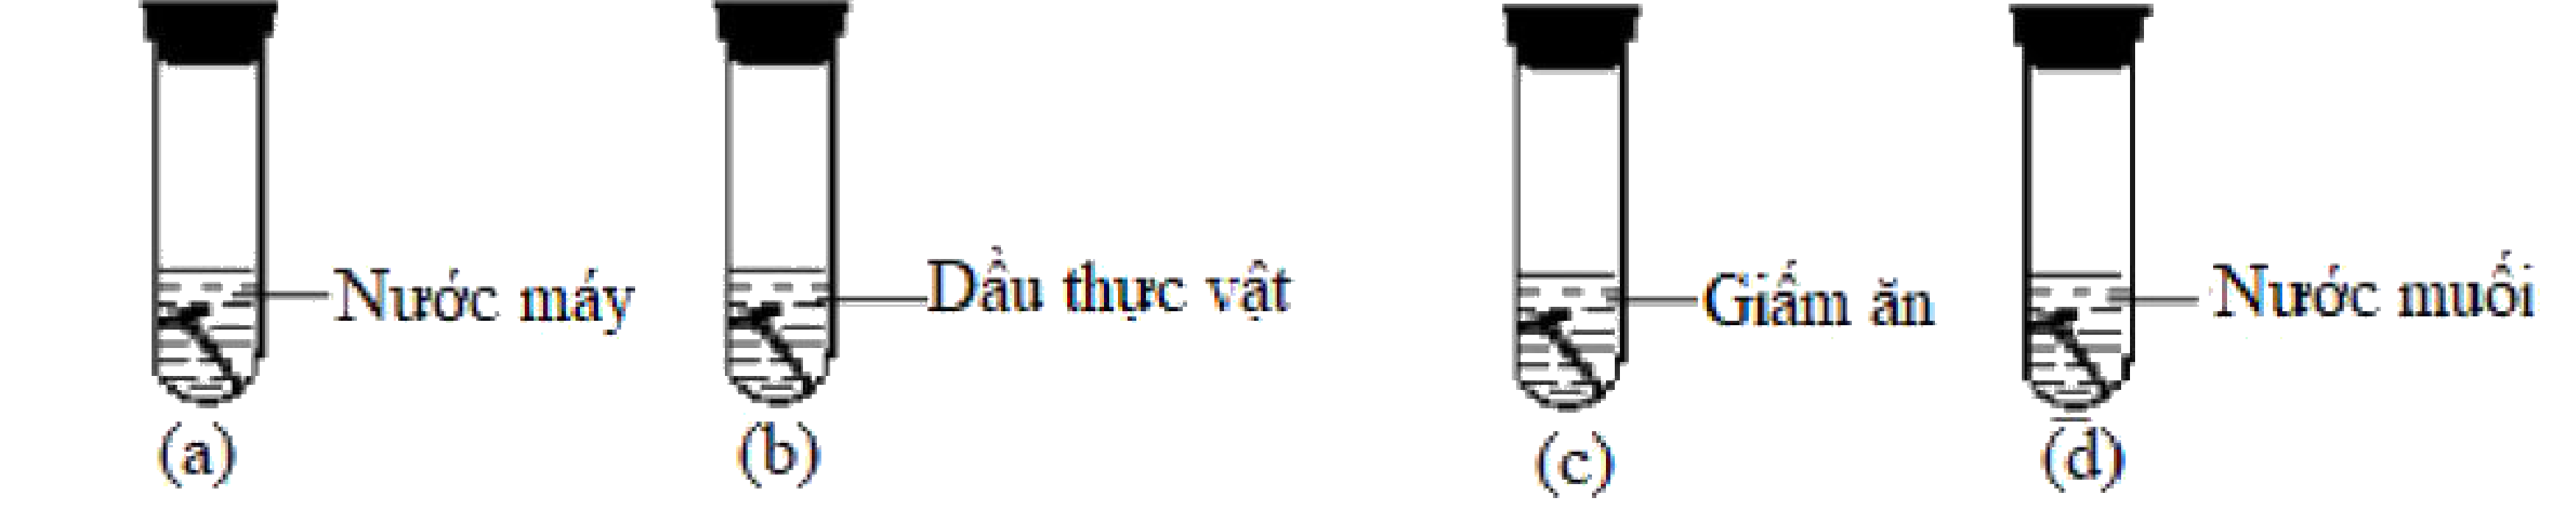
\includegraphics[height=1.1cm]{images_crop_de18/p1_cau17_bon_ong_nghiem.png}}\vspace{1pt}
\choice
{(a).}
{(b).}
{(c).}
{(d).}
\loigiai{}
\end{ex}

\begin{ex}
Tiến hành thí nghiệm của ba kim loại khác nhau với dung dịch hydrochloric acid loãng theo hình vẽ sau:
\par\vspace{1pt}\centerline{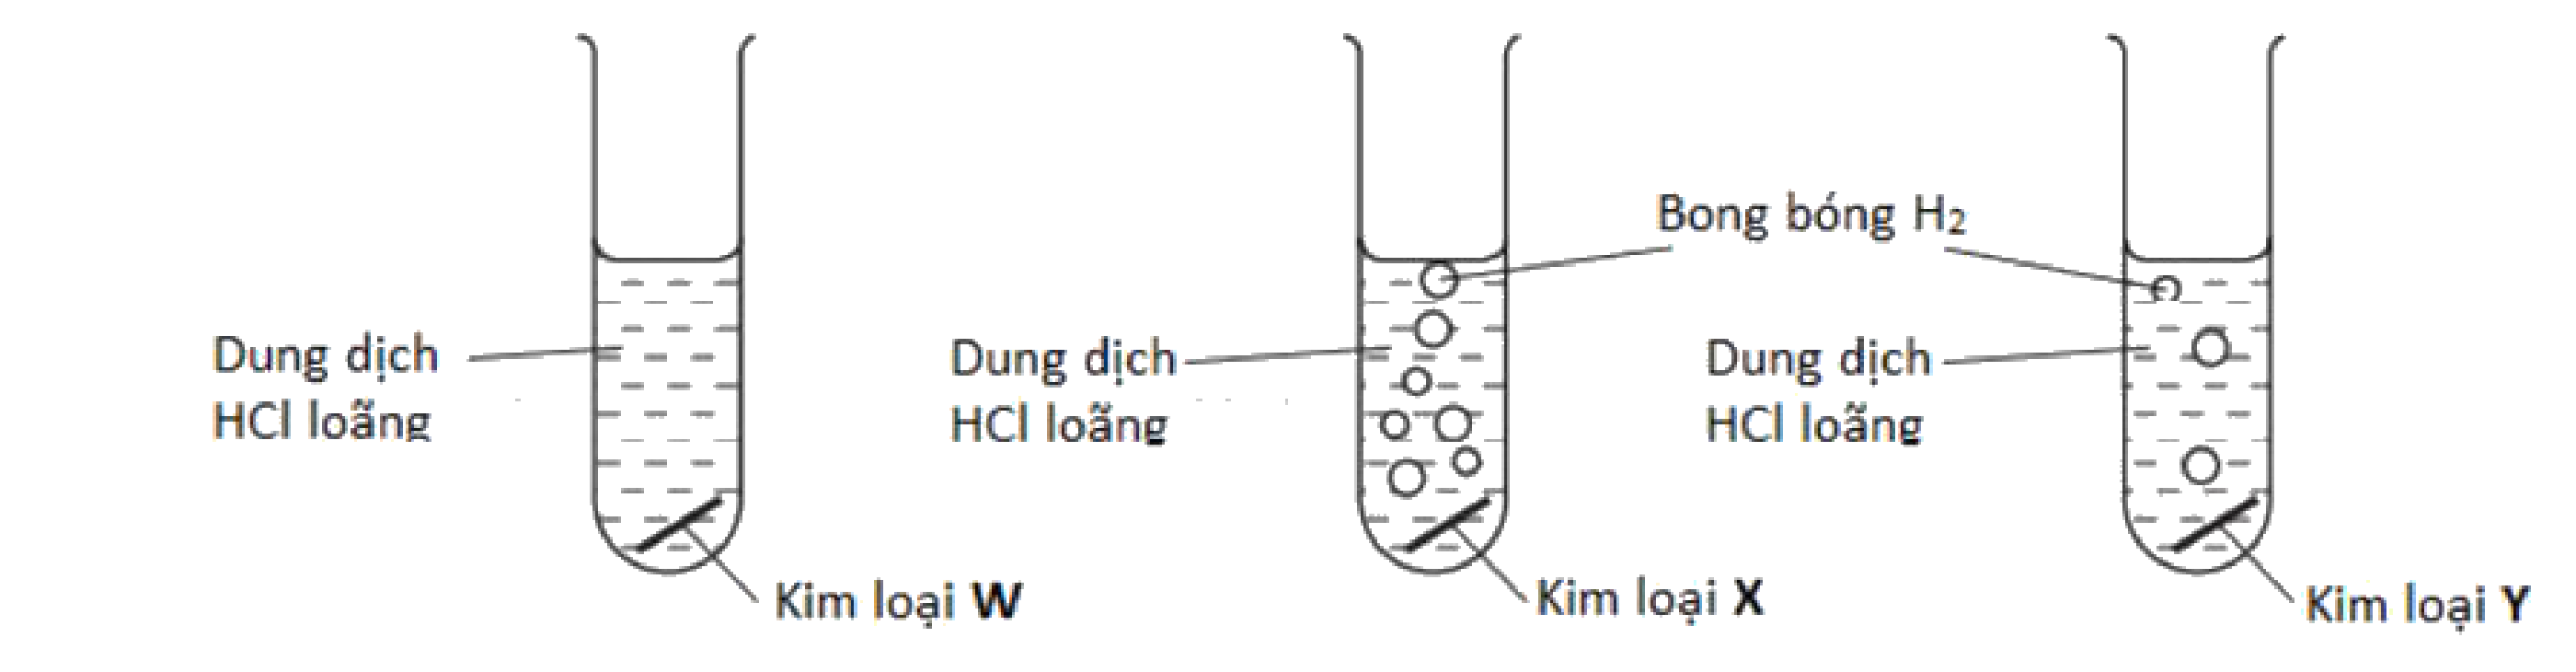
\includegraphics[height=1.2cm]{images_crop_de18/p1_cau18_ba_kim_loai_hcl.png}}\vspace{1pt}
Xác định các kim loại phù hợp với hình vẽ (theo thứ tự: Kim loại W, Kim loại X, Kim loại Y)?
\choice
{Cu, Mg, Zn.}
{Zn, Mg, Cu.}
{Mg, Zn, Cu.}
{Cu, Zn, Mg.}
\loigiai{}
\end{ex}

\newpage

\noindent
\textbf{PHẦN II (4,0 điểm -- 4 câu): Câu trắc nghiệm đúng sai.}\\
\textit{Thí sinh trả lời từ câu 1 đến câu 4. Trong mỗi ý a), b), c), d) ở mỗi câu, thí sinh chọn đúng hoặc sai.}

\setcounter{ex}{0}

\begin{ex}
Kim loại Cu có độ dẫn điện kém hơn Ag, kim loại Al có độ dẫn điện kém hơn Au nhưng dây dẫn điện chủ yếu làm bằng kim loại Cu và Al mà không phải là Ag và Au. Ứng dụng làm dây dẫn điện của Cu và Al là do chúng
\choiceTF
{đều dẫn điện tốt.}
{có giá thành phù hợp với thị trường tiêu dùng.}
{sản xuất được với quy mô công nghiệp.}
{đều có khối lượng riêng nhỏ.}
\loigiai{}
\end{ex}

\begin{ex}
Tiến hành thí nghiệm theo các bước sau:\\
\textbf{Bước 1.} Cho vào 3 ống nghiệm, mỗi ống 2 mL dung dịch \ce{H2SO4} 1 M.\\
\textbf{Bước 2.} Cho 3 lá kim loại có kích thước như nhau gồm lá nhôm (Al) đã làm sạch lớp bề mặt vào ống nghiệm (1), lá sắt (iron, Fe) vào ống nghiệm (2) và lá đồng (Cu) vào ống nghiệm (3).\\
Biết: $E^\circ_{\ce{Al^3+/Al}} = -1{,}676\text{ V}$; $E^\circ_{\ce{Fe^2+/Fe}} = -0{,}440\text{ V}$; $E^\circ_{\ce{Cu^2+/Cu}} = +0{,}340\text{ V}$.
\choiceTF
{Ở bước 2, ở cả ba ống nghiệm đều có khí thoát ra.}
{Tốc độ thoát khí ở ống (1) nhanh hơn ống (2).}
{Nếu thay \ce{H2SO4} loãng bằng \ce{H2SO4} đặc thì hiện tượng ở bước 2 sẽ không đổi.}
{Ở bước 2, nếu thêm tiếp 2 mL \ce{H2SO4} 1 M vào cả 3 ống thì tốc độ thoát khí ở cả ba ống sẽ tăng.}
\loigiai{}
\end{ex}

\begin{ex}
Nhôm phế liệu thường lẫn các tạp chất là các chất hữu cơ và vô cơ (có trong nhãn, mác do in hoặc sơn). Khi tái chế, phế liệu được cắt, băm nhỏ rồi cho vào lò nung đến khi chảy lỏng. Phần lớn các tạp chất này biến thành xỉ lỏng, nổi lên và được vớt ra khỏi lò. Phần còn lại là nhôm tái chế ở trạng thái lỏng và được đưa vào đúc khuôn.
\choiceTF
{Việc tái chế nhôm giúp giảm giá thành sản phẩm.}
{Việc tái chế nhôm giúp giảm chất thải ra môi trường.}
{Không nên dùng nhôm tái chế để chế tạo dụng cụ nhà bếp và y tế.}
{Đem cắt, băm nhỏ nhôm phế liệu để quá trình khử \ce{Al2O3} xảy ra dễ hơn.}
\loigiai{}
\end{ex}

\begin{ex}
Tiến hành thí nghiệm theo các bước sau:\\
\textbf{Bước 1.} Cho vào cốc thuỷ tinh 30 mL dung dịch \ce{H2SO4} 0,5 M.\\
\textbf{Bước 2.} Cho một lá nhôm và một lá đồng vào cốc sao cho chúng không tiếp xúc với nhau. Để yên khoảng 1 phút.\\
\textbf{Bước 3.} Dùng dây dẫn điện nối lá nhôm và lá đồng với một vôn kế (như hình bên).\\
Biết: $E^\circ_{\ce{Al^3+/Al}} = -1{,}676\text{ V}$; $E^\circ_{\ce{2H+/H2}} = 0\text{ V}$; $E^\circ_{\ce{Cu^2+/Cu}} = +0{,}340\text{ V}$.
\par\vspace{1pt}\centerline{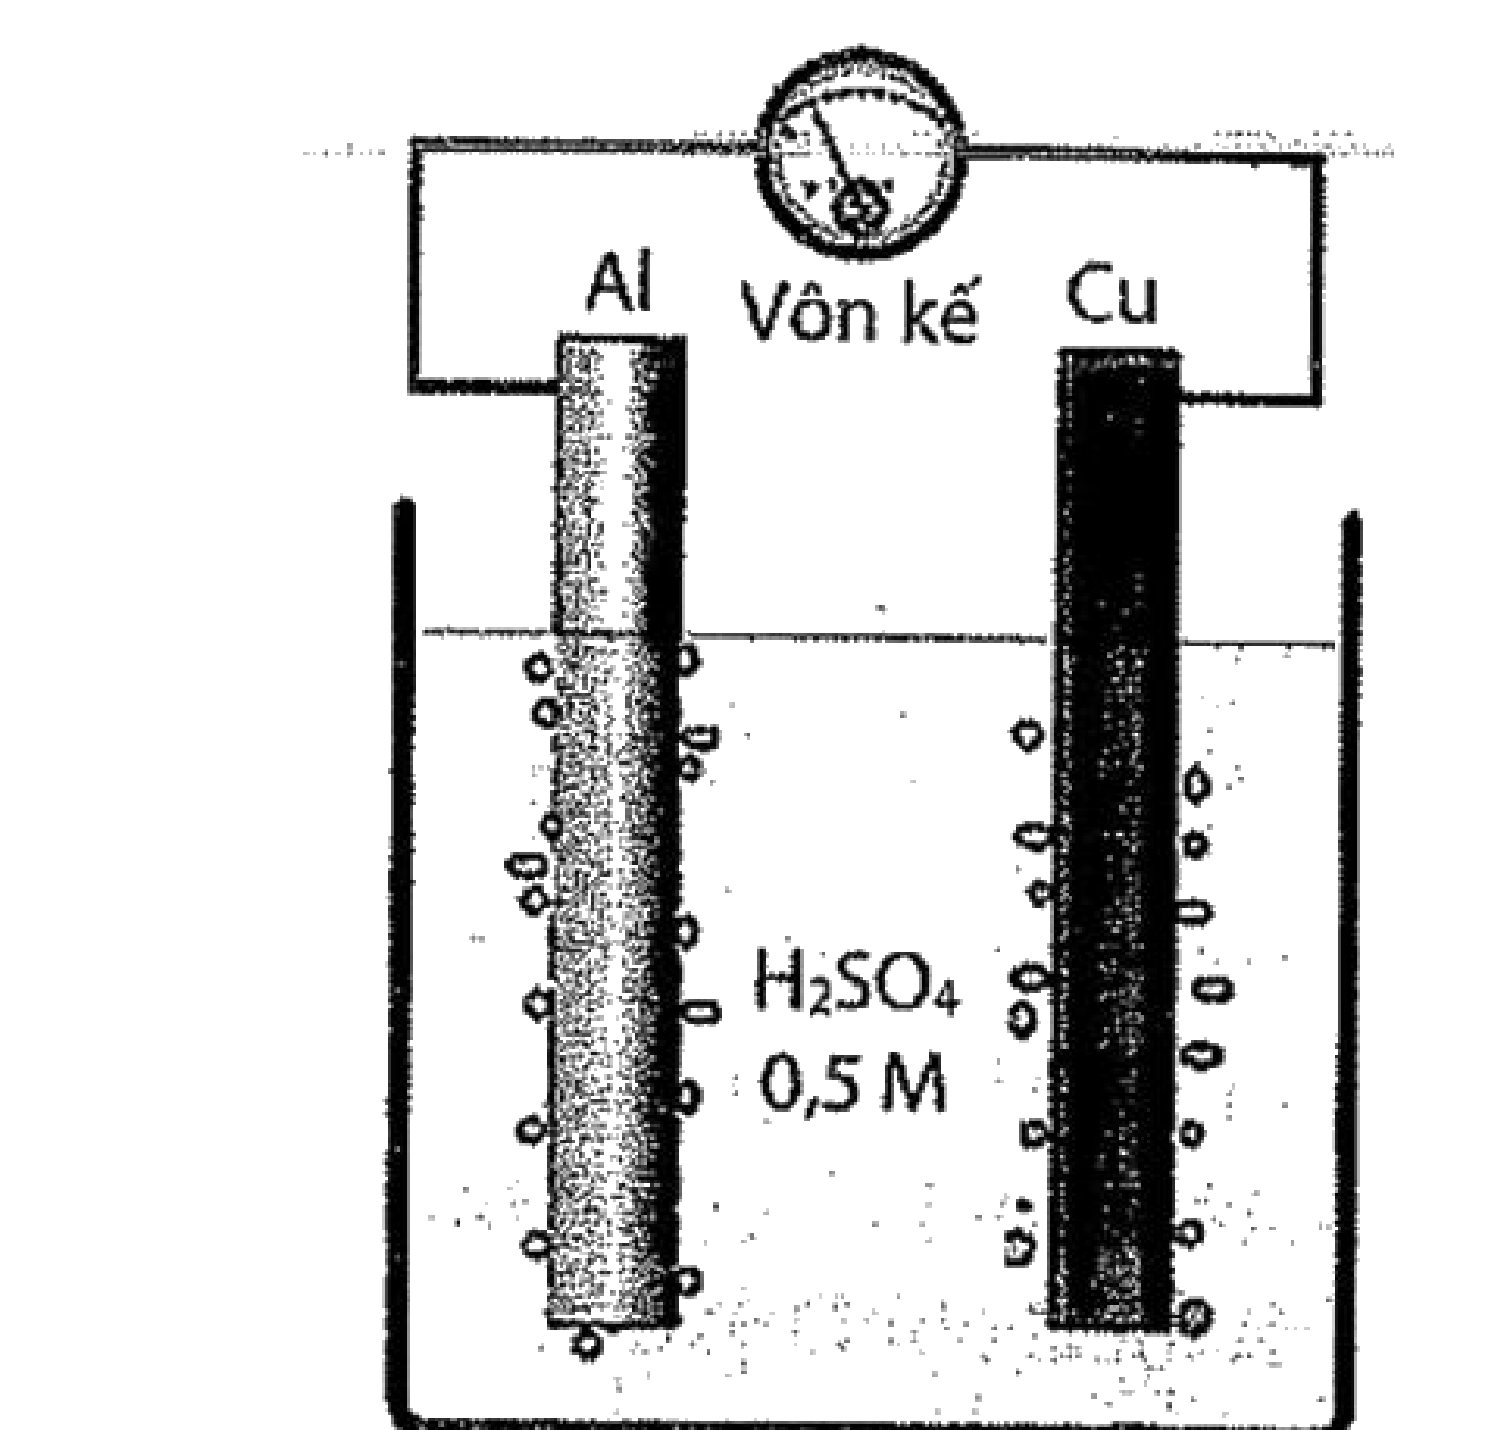
\includegraphics[height=2.2cm]{images_crop_de18/p2_cau4_pin_al_cu.png}}\vspace{1pt}
\choiceTF
{Ở bước 2, lá nhôm bị ăn mòn hoá học còn lá đồng không bị ăn mòn.}
{Ở bước 3, có sự tạo thành cặp pin điện hoá, trong đó lá nhôm là cathode và lá đồng là anode.}
{Ở bước 3, khí chỉ thoát ra ở bề mặt lá đồng, còn ở lá nhôm không có khí thoát ra.}
{Ở bước 3, kim vôn kế chỉ 1,336 V.}
\loigiai{}
\end{ex}

\newpage

\noindent
\textbf{PHẦN III (1,5 điểm -- 6 câu): Câu trắc nghiệm yêu cầu trả lời ngắn.}\\
\textit{Thí sinh trả lời từ câu 1 đến câu 6.}

\setcounter{ex}{0}

\begin{ex}
Quá trình sản xuất gang từ nguyên liệu quặng hematite, than cốc, chất chảy trong lò cao xảy ra các phản ứng chính:
\par\vspace{1pt}{\centering
\footnotesize\renewcommand{\arraystretch}{0.88}
\begin{tabular}{|c|l||c|l|}
\hline
\textbf{Nhiệt độ} & \textbf{Phương trình phản ứng} & \textbf{Nhiệt độ} & \textbf{Phương trình phản ứng} \\
\hline
$400^\circ\text{C}$ & $\ce{3Fe2O3 + CO ->[t^\circ] 2Fe3O4 + CO2}$ & $1300^\circ\text{C}$ & $\ce{CaO + SiO2 ->[t^\circ] CaSiO3}$ \\
$500 - 600^\circ\text{C}$ & $\ce{Fe3O4 + CO ->[t^\circ] 3FeO + CO2}$ & $1500^\circ\text{C}$ & $\ce{C + CO2 ->[t^\circ] 2CO}$ \\
$700 - 800^\circ\text{C}$ & $\ce{FeO + CO ->[t^\circ] Fe + CO2}$ & $1800^\circ\text{C}$ & $\ce{C + O2 ->[t^\circ] CO2}$ \\
$1000^\circ\text{C}$ & $\ce{CaCO3 ->[t^\circ] CaO + CO2}$ & & \\
\hline
\end{tabular}\par}\vspace{1pt}
Trong các phản ứng trên có bao nhiêu phản ứng oxi hoá -- khử?
\par\noindent\textit{Trả lời:} \dotfill
\loigiai{}
\end{ex}

\begin{ex}
Để bảo vệ vật bằng thép khỏi bị ăn mòn điện hoá, trong thực tế người ta đã thực hiện một số cách sau:\\
(1) Sơn kín bề mặt cánh cửa làm bằng thép.\\
(2) Tráng kẽm lên tấm thép mỏng khi sản xuất tôn.\\
(3) Gắn một số tấm kẽm lên vỏ tàu làm bằng thép.\\
(4) Cho dầu mỡ lên các ốc vít trên đường ray.\\
Liệt kê những cách sử dụng phương pháp bảo vệ bề mặt theo số thứ tự tăng dần.
\par\noindent\textit{Trả lời:} \dotfill
\loigiai{}
\end{ex}

\begin{ex}
Cho các tính chất vật lí ở cột (A) và giải thích ở cột (B) như sau:
\par\vspace{1pt}{\centering
\footnotesize\renewcommand{\arraystretch}{0.88}
\begin{tabular}{|l|p{12.2cm}|}
\hline
\textbf{Cột A} & \textbf{Cột B (Giải thích)} \\
\hline
(a) Tính dẻo & (1) Dưới tác dụng của điện trường, các electron tự do chuyển động có hướng. \\
(b) Tính dẫn điện & (2) Các electron tự do phản xạ ánh sáng nhìn thấy. \\
(c) Tính dẫn nhiệt & (3) Do các electron tự do liên kết các ion kim loại khi bị biến dạng cơ học. \\
(d) Tính ánh kim & (4) Các electron ở nhiệt độ cao truyền năng lượng cho ion dương và electron khác. \\
\hline
\end{tabular}\par}\vspace{1pt}
Hãy sắp xếp thứ tự giải thích của cột B với thứ tự tính chất vật lí ở cột A cho phù hợp.
\par\noindent\textit{Trả lời:} \dotfill
\loigiai{}
\end{ex}

\begin{ex}
Nhôm (Al) là kim loại phổ biến nhất trong vỏ Trái Đất. Nhôm được sử dụng để chế tạo hợp kim nhẹ, bền, được dùng trong kĩ thuật hàng không, trong xây dựng và làm nội thất. Nhôm có số hiệu nguyên tử là 13 và $E^\circ_{\ce{Al^3+/Al}} = -1{,}676\text{ V}$. Cho các phát biểu sau:\\
(1) Nhôm và đồ vật làm bằng nhôm dễ bị ăn mòn trong không khí ẩm.\\
(2) Ở trạng thái cơ bản, nguyên tử Al có 1 electron ở lớp ngoài cùng.\\
(3) Nhôm phản ứng được với nước ngay ở điều kiện chuẩn.\\
(4) Nhôm có tính khử mạnh hơn Mg (biết $E^\circ_{\ce{Mg^2+/Mg}} = -2{,}356\text{ V}$).\\
(5) Trong vỏ Trái Đất, nhôm chỉ tồn tại ở dạng hợp chất.\\
Liệt kê các phát biểu đúng theo số thứ tự tăng dần.
\par\noindent\textit{Trả lời:} \dotfill
\loigiai{}
\end{ex}

\begin{ex}
Để mạ đồng một vật dụng kim loại có diện tích $10\text{ cm}^2$, người ta điện phân dung dịch \ce{CuSO4} với cực âm là vật mạ và cực dương là lá đồng thô ($I = 2\text{ A}$, hiệu suất điện phân $90\%$, $D_{\ce{Cu}} = 8{,}94\text{ g/cm}^3$). Khối lượng đồng tính theo công thức Faraday: $m = \frac{A \cdot I \cdot t}{n \cdot F}$ ($A_{\ce{Cu}} = 64$, $F = 96485\text{ C/mol}$, $n = 2$). Thời gian điện phân để lớp mạ có độ dày $0{,}1\text{ mm}$ là bao nhiêu phút? (Làm tròn đến hàng đơn vị)
\par\noindent\textit{Trả lời:} \dotfill
\loigiai{}
\end{ex}

\begin{ex}
Đồng thau là hợp kim của đồng và kẽm. Để xác định hàm lượng Cu trong đồng thau, người ta cho 10 gam mảnh đồng thau vào dung dịch \ce{H2SO4} loãng dư; sau phản ứng hoàn toàn, lọc lấy chất rắn làm khô cân được 6,5 gam chất rắn. Hàm lượng đồng trong loại đồng thau trên bằng bao nhiêu \%? (Làm tròn đến hàng phần mười)
\par\noindent\textit{Trả lời:} \dotfill
\loigiai{}
\end{ex}


\Closesolutionfile{ans}
\end{document}
